\section{Results I: certificates on ground truth}
\label{sec:results-certificates}

This section reports the four audits on declared, exactly known models---the regime where the framework's claims are sharpest, because everything it certifies can be checked against ground truth. Experiments are labeled E1--E6 as in the repository. Positive and negative registered verdicts appear together; the negatives are then given their own treatment in Section~\ref{sec:negatives}.

\subsection{Coverage: the residual computes the right object (E1, E3)}
\label{sec:results-coverage}

\paragraph{Theorem anchors.} The chain-rule identity $\Xi(D \mid L \cup M) = \Xires - \mathrm{discharge}(M \mid L, D)$ holds with identically zero discrepancy in exact rational arithmetic on the tested models, and $\delta \le \varepsilon$ holds on every model built (both \gTheorem; the anchoring tests are named in Section~\ref{sec:repro}). % C-06, C-07, F-162

\paragraph{Residuals and ablations.} Full-schedule residual traces (\gExact): $\operatorname{tr}\Xi = 0.0837$ for REP(3), $0.0740$ for REP(5), $0.1754$ for SURF(3). % F-041 (C-08)
Dropping any single check strictly increases the residual, and REP(5)'s end-check drops differ from middle-check drops as registered (mean residual \emph{increase} on dropping one check: end $0.0593$ vs.\ middle $0.0204$; \gRegPos). % F-042, F-002 (C-09)
Duplicated checks show exactly zero discharge in both the E1 and E3 forms (\gRegPos)---the saturation null holding exactly, as the theory requires. % F-004, F-011 (C-12)

\paragraph{The single cleanest result: the degree ladder attains the exact optimum.} For REP(3) under N1, extend the native checks to the complete degree-2 family (all pairwise XOR products). The residual trace contracts from $0.083680$ to $0.027575$ (Figure~\ref{fig:ladder}), and the latter equals the \emph{enumerated optimal-decoder} mean squared error \emph{exactly}: both are the rational number $47291/1715000$, and the artifact records a difference of exactly $0.0$ (\gExact). % F-046 (C-10)
The registered prediction that the top rung equals the exact MMSE therefore held (\gRegPos). % F-010 (C-10)
The reason this is exact rather than merely close: the complete degree-2 family generates every function of the syndrome for REP(3), so the linear-estimator floor over that family \emph{is} the true optimal-decoder MMSE. This is the paper's sharpest instance of ``the audit computes the right object'': a coverage certificate derived from SBT's chain-rule formalism lands, digit-for-digit as a fraction, on the quantity a QEC practitioner would compute by brute-force enumeration. We permit ourselves the word ``optimal'' for this result because it literally attains the enumerated optimum; everywhere else in this paper the word appears only inside the standard names of mathematical objects (the coverage-optimal map $A^{*}$, the enumerated optimal-decoder MMSE, the minimal machine that acts optimally) or as a by-construction property of the first greedy step, never as a performance claim.

\begin{figure}[htbp]
\centering
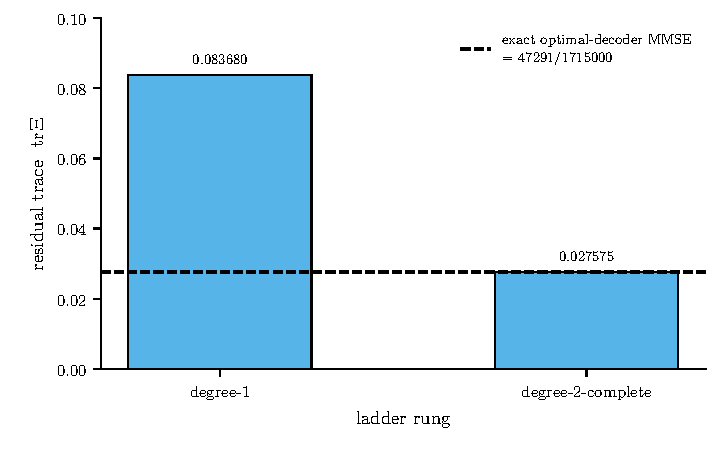
\includegraphics{figures/generated/fig_F4_e3_degree_ladder.pdf}
\caption{Degree-ladder contraction on REP(3) under N1 (E3). The degree-2-complete rung's residual equals the enumerated optimal-decoder MMSE exactly: both are $47291/1715000$, and the recorded difference is exactly $0.0$ (\gExact). The complete degree-2 family generates every function of the REP(3) syndrome, so its linear-estimator floor \emph{is} the true optimal-decoder MMSE, not an approximation to it.}% F-046, F-010 (C-10)
\label{fig:ladder}
\end{figure}

\paragraph{Selection beats baselines at every budget.} On SURF(3), greedy chain-rule check selection contracts the residual from the no-check baseline $0.4345$ to the full-schedule $0.1754$, and at \emph{every} intermediate budget its residual is at or below every tested baseline (lexicographic order and 10 seeded random orders; Figure~\ref{fig:budget}; \gRegPos). % F-044, F-045, F-009 (C-11)
This is a registered comparison against the tested baselines, not a general optimality statement: only the first greedy step is optimal by construction. Greedy selection carries the classical $(1-1/e)$ guarantee only for submodular objectives~\cite{nemhauser1978greedy,krause2008sensor}, and variance reduction by a set of regressors is not submodular in general~\cite{das2011submodular}, so no such guarantee is claimed here. The greedy selector also stops before exhausting a duplicate-padded candidate list rather than spending budget on provably worthless checks (\gRegPos). % F-012

\begin{figure}[htbp]
\centering
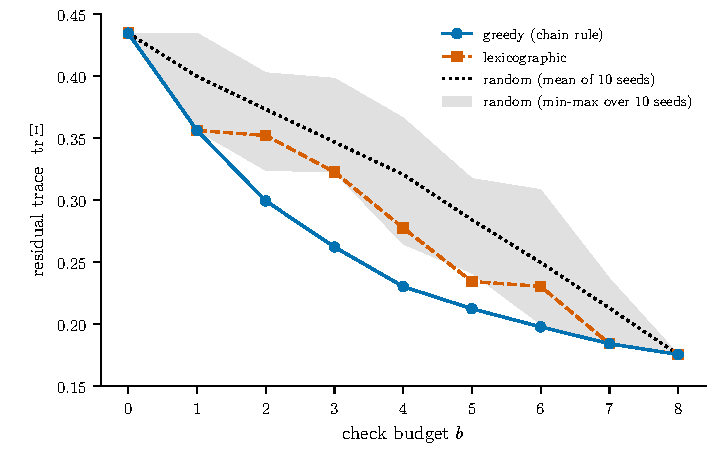
\includegraphics{figures/generated/fig_F3_e3_coverage_vs_budget.pdf}
\caption{Residual trace versus check budget under chain-rule greedy selection on SURF(3) (E3). Greedy is at or below the lexicographic order and every one of 10 seeded random orders at every budget (\gRegPos). This is a comparison against the tested baselines, not a general optimality statement: only the $b = 1$ step is optimal by construction.}% F-044, F-045, F-009 (C-11)
\label{fig:budget}
\end{figure}

\subsection{Existence: the certificate does classification work (E4)}
\label{sec:results-existence}

The typed existence certificate was computed on ground-truth Markov cycle models (\gExact{} for the REP rows). The baseline package---REP(3), N1 noise, the standard decoder---certifies: $\delta = 0.007144875$, $\varepsilon = 0.00725$ (the theorem bound $\delta \le \varepsilon$ visibly tight), multiplicity 2, status \texttt{certified}. % F-048 (C-13)
The deliberately broken decoder (mapping everything to one logical state) is caught by the multiplicity guard: $\delta = 0$ \emph{exactly}---perfect idempotence---but multiplicity 1 and status \texttt{trivialized} (\gRegPos{} for the guard). % F-049, F-016 (C-13, C-14)
This pair is the certificate idea in one contrast: a small idempotence defect alone would have certified the broken decoder; the typed certificate refuses. Sweeping the physical error rate under the sweep's defect-only rule (status \texttt{degrading} once $\delta$ exceeds $0.05$) flips the label from \texttt{certified} to \texttt{degrading} at $p = 1/5$ ($\delta$ rising monotonically $0.000298 \to 0.007145 \to 0.026432 \to 0.082368$ across $p \in \{1/100, 1/20, 1/10, 1/5\}$; \gExact). % F-050 (C-13)
At $p = 1/5$ the full typed classifier would return \texttt{trivialized} rather than \texttt{degrading}: no prototype remains stable there (multiplicity $0$, $\varepsilon = 0.104$), and multiplicity takes priority over the defect threshold (\gExact). % F-166 (C-13)
Table~\ref{tab:certificate} collects the classification.

\begin{table}[htbp]
\centering\footnotesize\setlength{\tabcolsep}{4pt}
\begin{tabular}{l r r r l}
\toprule
package & $\delta$ & $\varepsilon$ & mult. & status \\
\midrule
REP(3) + N1, standard decoder, $p = 1/20$ & 0.007144875 & 0.00725 & 2 & \texttt{certified} \\ % F-048
same, deliberately broken decoder & 0 (exact) & 0 & 1 & \texttt{trivialized} \\ % F-049
same, $p = 1/5$ (sweep rule) & 0.082368 & 0.104 & 0 & \texttt{degrading}$^{\dagger}$ \\ % F-050, F-166
\bottomrule
\end{tabular}
\caption{The existence certificate doing classification work on ground truth (\gExact). The broken decoder has \emph{perfect} idempotence---the multiplicity guard, not the defect, is what catches it. The remaining status, \texttt{non\_closed}, is thresholded on the closure deficit; its registered demonstration on the hidden-mode model was a \gRegNeg{} discussed in Appendix~\ref{app:predictions} (P4.2: the zero-deficit clause holds on the syndrome lens, not the frozen decoded lens). $^{\dagger}$The sweep assigns its label from the defect threshold alone; with multiplicity $0$ the full classifier would return \texttt{trivialized} at $p = 1/5$.} % F-048, F-049, F-050, F-014
\label{tab:certificate}
\end{table}

Two further certificate components behaved as designed on hidden-state models. The closure deficit correlates with an out-of-sample predictive gap across the model/horizon grid: Pearson $r = 0.936$ with the latching model N5 included (\gMeasured). % F-054 (C-15)
The registered bar $r \ge 0.9$ held (\gRegPos). % F-017 (C-15)
The same computation without N5 gives $r = -0.171$, which we report alongside; restricted to that narrow slice the registered correlation does not hold. % F-054 (C-15)
And the route-mismatch diagnostic exhibits the intended leakage signature on N5---a decoder lens that remains channel-accurate ($0.75$) while $RM$ grows severalfold over horizon (peak ratio $7.28\times$ baseline)---though it saturates below the frozen $10\times$ bar, a \gRegNeg{} discussed in Section~\ref{sec:negatives}. % F-052 (P4.3)

\subsection{Memory: exact witnesses, a genuine payoff, and a control that fired on us (E5)}
\label{sec:results-memory}

\paragraph{Witnesses separate the family exactly.} On the memoryless package (N1), the predictive-quotient audit finds \emph{zero} memory witnesses ($|Q| = |M| = 4$, $\Delta^{\max} = 0$; \gExact). On the hidden-mode package (N4) it finds 4 witnesses, MaxFiber 2, and an exact worst-case predictive gap $\Delta^{\max} = 112329952/1318359375 \approx 0.0852$; on the latching package (N5), 4 witnesses with $\Delta^{\max} = 539/1250 = 0.4312$ (\gExact). % F-028, F-029, F-030 (C-16)
These are certificates in the strict sense: exact rational statements that, within the declared catalog of histories, events, and continuations, currently indistinguishable histories assign different probabilities to some declared future event on N4/N5---by at most $\Delta^{\max}$---and identical probabilities on N1. Whether a decoder can turn that difference into performance is the separate, measured question below.

\paragraph{Currentization names the hidden coordinate.} Adding the mode bit as an observable dissolves the predictive surplus at candidate-set cardinality 1; no set of pure check bits does (\gRegPos). % F-021 (C-17)
The audit does not merely detect hidden memory---it identifies \emph{which} added observable would expose it.

\paragraph{The protocol trap fired against our hypothesis.} We built a two-phase alternating noise schedule as the intended ``schedule artifact,'' registering the prediction that internalizing the schedule (adding the phase as an autonomous state coordinate) would dissolve its witnesses, classifying it \texttt{artifact\_trap}. That prediction \emph{failed} as registered: internalization preserved all 4 witnesses and the package classifies \texttt{genuine\_memory\_after\_internalization} (\gExact{} for the classification). % F-032, F-070 (C-20)
The registered artifact hypothesis therefore failed (\gRegNeg). % F-020 (C-20)
The reading (\gInterp): a deterministic $p_0$-vs-$3p_0$ alternation carries real predictive content---the current phase predicts next-round statistics---so the trap correctly declined to call it an artifact. We state this carefully because it is easy to misreport: the control mechanism worked, and what it falsified was \emph{our} registered ``this is an artifact'' hypothesis. This is a negative result for that hypothesis, not a demonstration of the trap catching an artifact. % C-20

\paragraph{Memory's measured value, under a proper scoring rule.} The frozen accuracy-based payoff comparison came back nil, for a reason the diagnosis identified exactly: under X-only noise at $p < 1/2$, mode-conditional MAP correction picks the same coset representative in every mode, so accuracy-scored decoders tie by construction. A post-registration study (separately labeled, leaving all frozen verdicts untouched) rescored predictors on next-round negative log-likelihood, a strictly proper scoring rule~\cite{gneiting2007proper} (Figure~\ref{fig:payoff}), where memory has room to show non-tautological value. Findings (\gMeasured): the exact Bayes filter~\cite{rabiner1989hmm}, which reads the full round outcome (both syndrome bits and the logical increment), captures $0.00196$ of the $0.01061$ nats/round oracle ceiling at the frozen defaults and $0.03615$ of $0.05834$ at a declared louder operating point. % F-034, F-037 (C-18)
We read these as about 18\% and 62\% of ceiling (\gInterp). % F-040
A \emph{declared 2-state} run-length machine---driven by a two-bit slice of the outcome record (one syndrome bit and the logical increment), trained on the first half of each trajectory and scored on the second---captures a positive share ($0.00015$ and $0.00429$ nats/round), rising with machine size $K$ at the frozen defaults and up to $K{=}8$ in loud mode, where $K{=}16$ sits slightly below $K{=}8$ ($0.01036$ vs.\ $0.01052$; \gMeasured). % F-035, F-038 (C-18)
Naive per-step rounding of the continuous belief coordinate is \emph{value-destroying} below a resolution threshold: negative at every tested resolution at the frozen defaults (and non-monotone there, worst at $K{=}4$: $-0.0047$, $-0.0062$, $-0.0053$, $-0.0037$ for $K = 2, 4, 8, 16$), and negative in loud mode except at $K{=}16$, where a positive $+0.0301$ contradicted our pre-stated all-negative expectation and is reported as such (\gMeasured). % F-036, F-039 (C-19)
The packaging-theoretic reading (\gInterp): summarizing a short run-length statistic of the outcome record is cheap and safe; quantizing an \emph{internal belief} has a resolution threshold below which it destroys value. The run-length and rounding gaps are scored on different windows (second half vs.\ full trajectory), so their magnitudes are compared only qualitatively.

\begin{figure}[htbp]
\centering
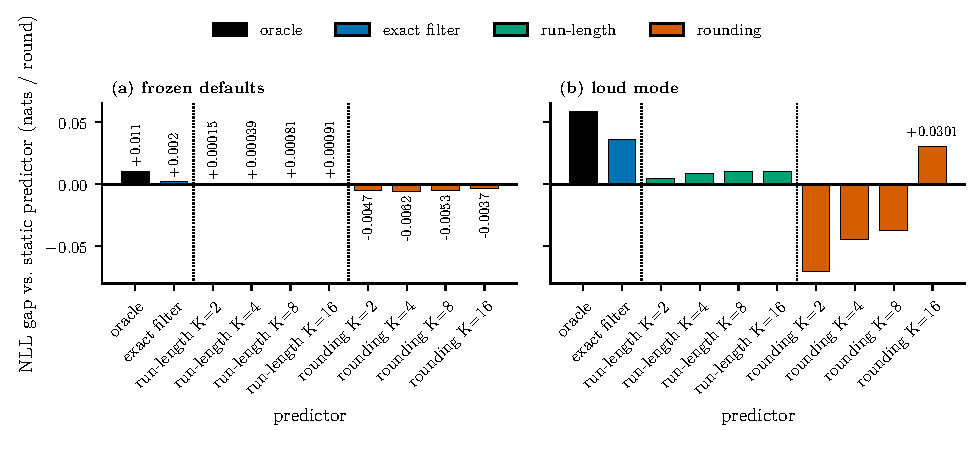
\includegraphics{figures/generated/fig_F5_e5_payoff_ladder.pdf}
\caption{Decoder-memory value under a proper scoring rule: next-round NLL gap over the static predictor on REP(3)+N4, at the frozen defaults (a) and the declared louder operating point (b) (E5, post-registration study; \gMeasured). The oracle is a ceiling, not deployable; the exact Bayes filter, which reads the full round outcome, is the realistic upper bound; run-length machines (driven by one syndrome bit and the logical increment, and scored on the second half of each trajectory while the other predictors are scored on the full trajectory) are positive and generally improve with $K$, with a slight loud-mode decline from $K{=}8$ to $K{=}16$; belief-rounding machines are value-destroying except the loud-mode $K{=}16$ point at $+0.0301$, a measured result reported as it stands, not an error bar. Values are printed beside the frozen-default bars, which are too small to read on the shared scale.}% F-034, F-035, F-036, F-037, F-038, F-039 (C-18, C-19)
\label{fig:payoff}
\end{figure}

\subsection{Pricing: exact machinery, negative evidence (E6)}
\label{sec:results-pricing}

The pricing audit is this paper's clean full negative, and we present it with the same prominence as the positives. The machinery itself is exact where declared and runs correctly: the exact value curve $V(b)$ by enumeration and the shadow-price curve $\lambda(b)$ (\gExact). % F-055, F-057 (C-21a)
The greedy selector's gap to the exact curve is at most $0.00405$ on REP(5) (\gMeasured). % F-056 (C-21a)
Every registered \emph{prediction} about pricing behavior failed at the frozen tolerances (\gRegNeg{} throughout): % C-21b
$\lambda$ was predicted nonincreasing after its maximum, and mixed degree-1/degree-2 costs instead produce sawtooth marginal values at budget parities; % F-022, F-071
a slack point $b^{*} < b_{\max}$ was predicted, and instead $b^{*} = b_{\max}$ for both code families because the frozen tolerance sits below the smallest genuine marginal value; % F-023, F-072
the consequence test (removing the last pre-slack unit should shift the sampled logical error rate detectably) did not separate: $\Delta = -0.000135$ against a combined standard error of $0.000119$; % F-059, F-073
and permuted proxy costs were strictly worse at only 36.9\% of budget points against a registered 80\% bar. % F-060, F-074
We do not soften this: as instantiated and thresholded here, the pricing primitive produced no positively evidenced result. The readings in Section~\ref{sec:negatives} suggest the failures are threshold-scale and test-design errors rather than refutations of the pricing concept (\gInterp), but on this prototype's evidence the primitive stands negative.

% ===========================================================================
